% !TEX spellcheck = en_US

% !TEX root = expose.tex

%%%%%%%%%%%%%%%%%%%%%%%%%%%%%%%%%%%%%%%%%%%%%%%%%%%%%%%%%
\begin{frame}

\maketitle
%\vspace{1cm}
%
%\centerline{\huge \textbf{CEMRACS Project Elasto$\Phi$}}\quad\\[-5pt]
%
%\quad\\\quad\\
%
%\centerline{{\large M.~Bonazzoli$^{\dagger}$, P.~Marchand$^{*}$, X.~Claeys$^{*}$,}}
%\centerline{{\large P.-H.~Tournier$^{*}$, I.~Ben-Gharbia$^{\S}$, F.~Nataf$^{*}$}}
%
%
%\quad\\
%\hspace{2.5cm}\begin{tabular}{l}
%{\small $^{\dagger}$ Labo.~J.A.~Dieudonn\'e, Univ.~Nice Sophia Antipolis, }\\
%{\small $^{*}$  INRIA Alpines / Labo.~J.-L.~Lions UPMC,}\\
%{\small $^{\S}$ IFP Energies Nouvelles.}
%\end{tabular}
%
%
%\vspace{1cm}


%\begin{picture}(-20,10)(-10,-25)
%  \put(40,25){      
%    \put(10,-75) {
\includegraphics[height=2cm]{../logo/logo_ljll.pdf}}
%    \put(70,-75){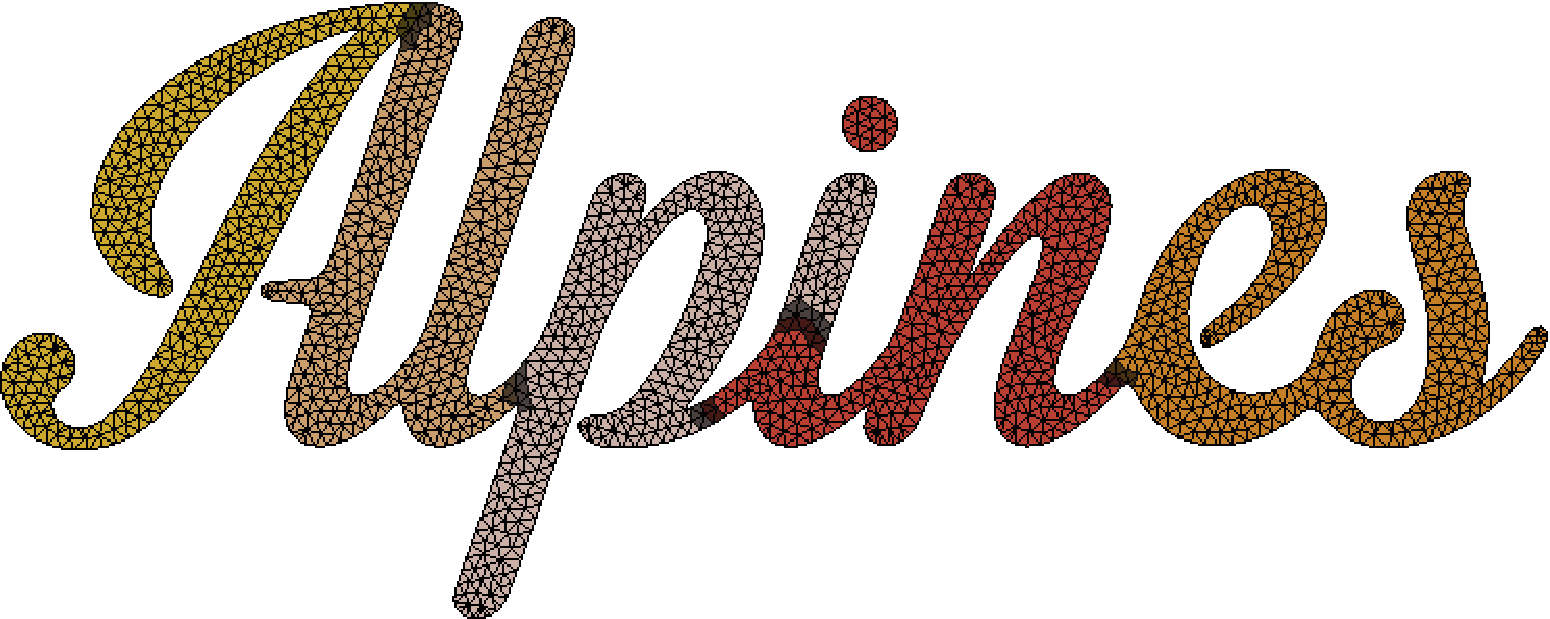
\includegraphics[height=1.75cm]{../logo/logo_alpines.pdf}}
%    \put(200,-75)  {
\includegraphics[height=2cm]{../logo/logo_anr.png}}
%    \put(10,-135)  {
\includegraphics[height=2cm]{../logo/logo_ifpen.pdf}}
%    \put(150,-135)  {
\includegraphics[height=2cm]{../logo/logo_unice.png}}
%  }
%\end{picture}

\end{frame}

%%%

\begin{frame}
\frametitle{The Elasto$\Phi$ project: the IFPEN problem} 
%\framesubtitle{}

Elastostatic problem in \alert{crack networks} of 2 types: 

geological \emph{fault} network and discrete \emph{fracture} network 

\vspace{-5pt}

\begin{figure}
\centering
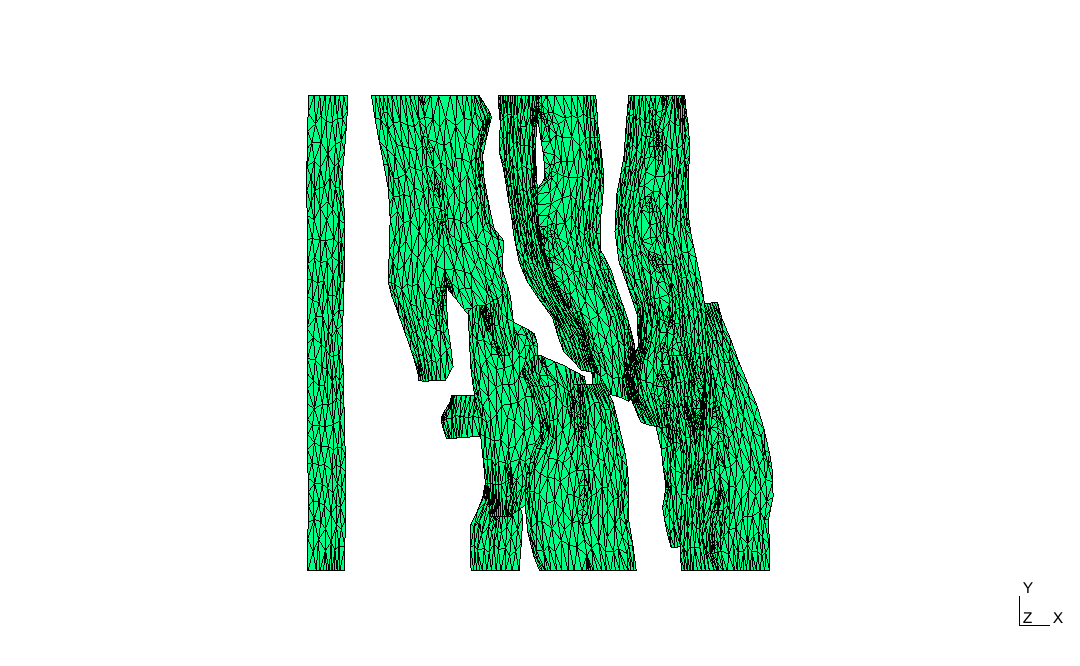
\includegraphics[width=0.35\textwidth]{../images/visu_maillage5364FracsTriangles.png} \quad
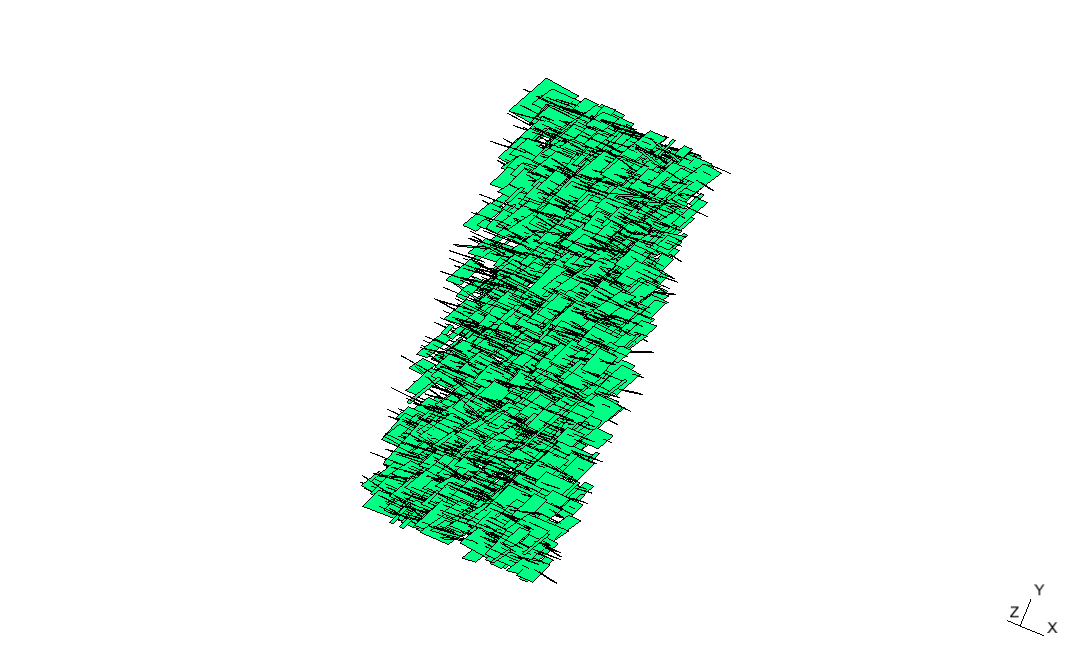
\includegraphics[width=0.25\textwidth]{../images/visu_maillage1994Fracs.png}
\end{figure}

Boundary \emph{integral equation} posed at the surface of cracks

$\Rightarrow$ \alert{dense matrix} $\mA\in \R^{n\times n}$
$\Rightarrow$ $\mathcal{O}(n^{2})$ for matrix-vector product.

\medskip
IFPEN heuristic approach to sparsify $\mA$ gives large error ($16$\%--$40$\%)

\end{frame}

%%%

\begin{frame}
\frametitle{The Elasto$\Phi$ project} 
%\framesubtitle{}

Many refined \emph{complexity reduction} techniques in current literature on boundary integral equation.

\bigskip
Two ingredients in the approach we considered: 
\begin{itemize}
\item
Adaptative Cross Approximation (\alert{ACA}),
\item
Hierarchical Matrices (\alert{HM}).
\end{itemize}

\medskip
Challenge: \emph{strongly irregular geometry!}

\bigskip
\bigskip

{\tiny
[M.~Bebendorf. Hierarchical matrices: A Means to Efficiently Solve Elliptic Boundary Value Problems, {\em Lecture Notes in Computational Science and Engineering}, 2008]

\smallskip
[S.~Rjasanow, O.~Steinbach. The fast solution of boundary integral equations. {\em Mathematical and Analytical Techniques with Applications to Engineering}, 2007.]

\smallskip
[W.~Hackbusch. Hierarchical Matrices: Algorithms and Analysis, {\em Springer Series in Computational Mathematics}, 2016.]

\smallskip
[S.~A.~Sauter, C.~Schwab. Boundary element methods, {\em Springer Series in Computational Mathematics}, 2011.]
\par} %\par per interlinea giusti

\end{frame}

%%%

\begin{frame}
\frametitle{Adaptative Cross approximation (ACA)}
\framesubtitle{The idea of the Singular Value Decomposition (SVD)} 
Suppose that $\mathrm{A} \in \R^{n\times n}$ is such that 
\[
\mA = \sum_{j=1}^{k}\bfu_{j}\cdot\bfv_{j}^{T}\quad \text{with}\quad k\leq n/2.
\]
$\Rightarrow$ $2kn$ operations

\bigskip
SVD actually gives the following decomposition:
\begin{equation*}\label{SVD}
\mA = \sum_{j=1}^{n}\sigma_{j}\,\bfu_{j}\cdot\bfv_{j}^{T}\quad \text{ where }\{\sigma_{j}^{2}\}_{j=1\dots n} \text{ are the eigenvalues of } \mA^{T}\mA,
\end{equation*}

But it costs $\mathcal{O}(n^{3})$ ...

\end{frame}

%%%

\begin{frame}
\frametitle{Adaptative Cross approximation (ACA)}
\framesubtitle{An approximation of the Singular Value Decomposition (SVD)} 
\begin{algorithm}[H]
  \caption{Partially Pivoted ACA}  
  \label{AlgoACA}
  Initialize $j_{*}$\\
  $r=0$\\
  \textbf{while}(stopping criterion not satisfied)\{\\
  \indent\hspace{0.5cm} \parbox{\linewidth}{
    $\bfw = \mA(j_{*},:)^{T} - \sum_{\ell=1}^{r}\bfu_{\ell}(j_{*})\,\bfv_{\ell}$\\
    $k_{*} = \mathop{\mrm{argmax}}_{k = 1\dots n}\vert \bfw(k)\vert$\\
    $w_{*} = \bfw(k_{*})$\\
    \textbf{if}($w_{*}\neq 0$)\{\\\quad\\
    \indent\hspace{0.5cm} \parbox{\linewidth}{
      $\bfv_{r+1} = \bfw$\\
      $\bfw = \mA(:,k_{*})-\sum_{\ell = 1}^{r}\bfv_{\ell}(k_{*})\,\bfu_{\ell} $\\
      $\bfu_{r+1} = w_{*}^{-1}\bfw$\\      
      $j_{*} = \mathop{\mrm{argmax}}_{j = 1\dots n} \vert \bfw(j)\vert$\\
      $r=r+1$
    }
   \}\\
    \textbf{else}\{terminate algorithm\}
    }\\
  \}

\end{algorithm}

\end{frame}

%%%

\begin{frame}
\frametitle{Adaptative Cross approximation (ACA)}
\framesubtitle{Comparaison between SVD and ACA} 
Compression of the interaction between two clusters of points
\begin{figure}
	\centering 
	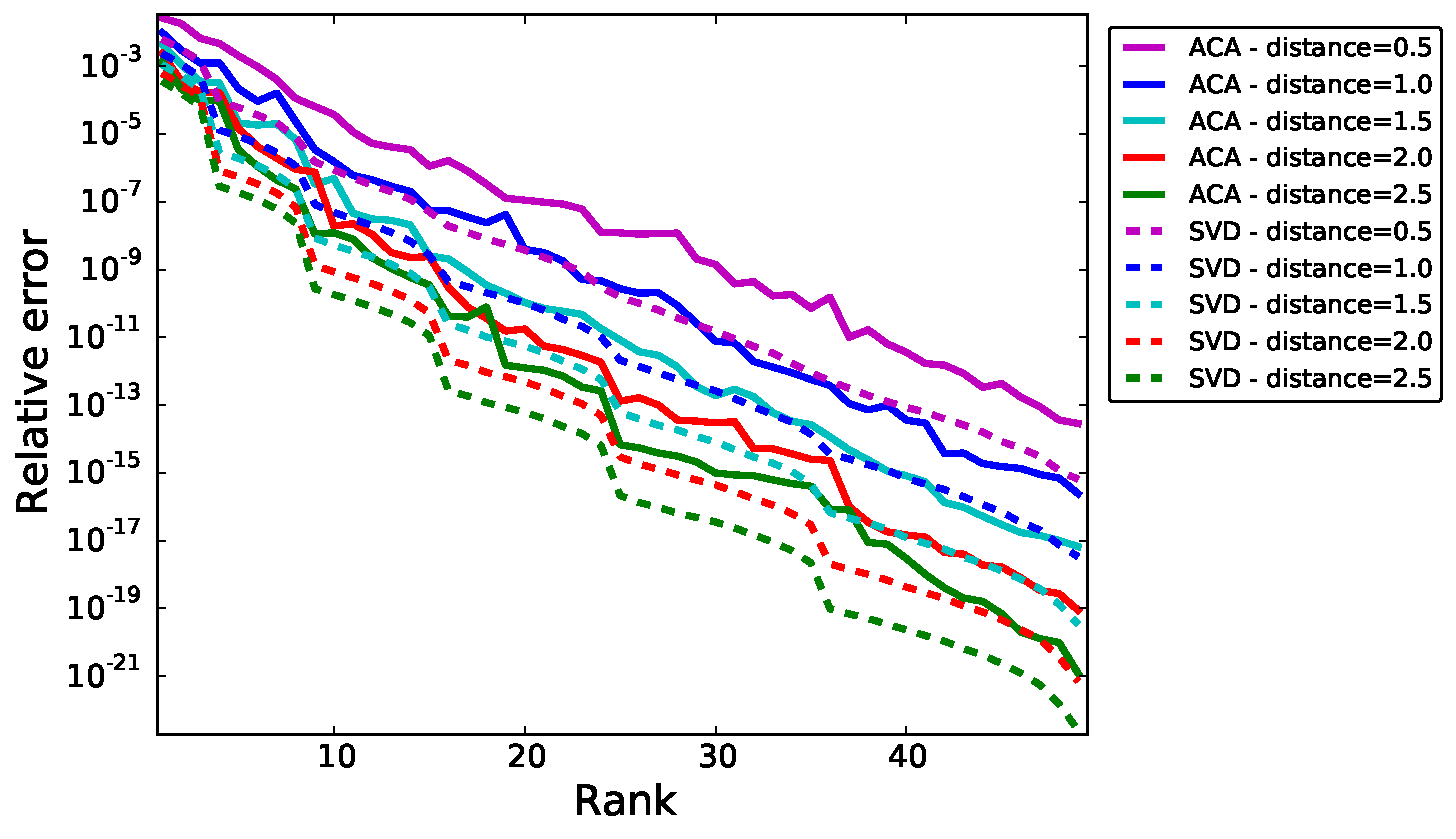
\includegraphics[width=0.9\textwidth]{../images/graphe_output_err_decrease}
\end{figure}


\end{frame}

%%%

\begin{frame}
\frametitle{Adaptative Cross approximation (ACA)}
\framesubtitle{In practice} 
The matrix comes from the discretization of a boundary integral equation 
\begin{equation*}\label{GalerkinMatrix}
\mA_{j,k}:= \int_{\tau\times\tau'}\mathscr{G}(\bx-\by) \bpsi_{j}(\bx)\bpsi_{k}(\by) d\sigma(\bx) d\sigma(\by),\quad j,k = 1\dots n.
\end{equation*}
$\mathscr{G}$ is an integral kernel such that 
\begin{itemize}
\item it is singular for $\bx = \by$, i.e~ if $\tau \cap \tau' \ne \emptyset$
\item it is regularizing if $\tau$ and $\tau'$ are distant from each other 
\end{itemize}
\bigskip

 $\Rightarrow$ ACA is applicable to sub-blocks of $\mA$ 
 
 $\Rightarrow$ Hierarchical matrices
\end{frame}

%%%

\begin{frame}
\frametitle{Hierarchical matrices}
We build a cluster tree representing the unknowns, example:
\begin{figure}
	\centering
	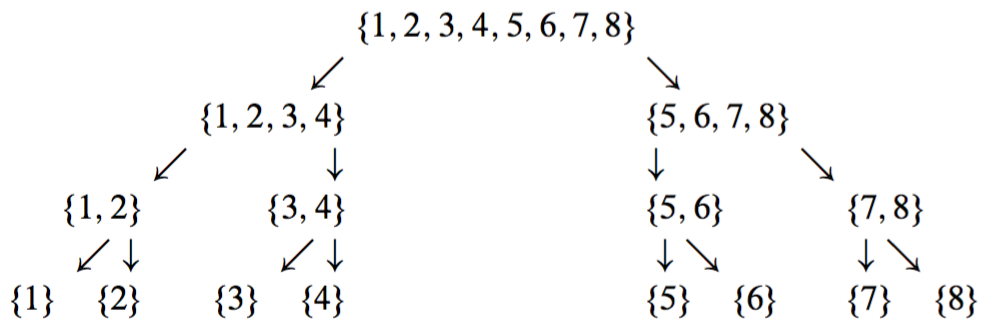
\includegraphics{../clustering}
	
	
\end{figure}


\end{frame}








